\documentclass{thesis}


% Settings
% Persian fonts
% Persian & English fonts (LOCAL FONT FILES)
% Font files are stored in /fonts directory


\settextfont[
Path=fonts/,
Extension=.ttf,
UprightFont=* ,
BoldFont=*Bold
]{BNazanin}


\setlatintextfont[
  Path=fonts/,
  Extension=.ttf,
  UprightFont=*,
  BoldFont=*Bold,
  ItalicFont=*Italic,
  BoldItalicFont=*BoldItalic
]{TimesNewRoman}


% Special font for thesis title
\newfontfamily\BTitr[
Path=fonts/,
Extension=.ttf
]{BTitr}


% Nastaliq font (for Bismillah page)
\newfontfamily\IranNastaliq[
Path=fonts/,
Extension=.ttf
]{IranNastaliq}


% 
% In fonts.tex
\settextfont[Path=fonts/, Extension=.ttf, UprightFont=*, BoldFont=*Bold]{BNazanin}
\newfontfamily\BNazaninFont[Path=fonts/, Extension=.ttf, UprightFont=*, BoldFont=*Bold]{BNazanin}

% in settings/fonts.tex
\newcommand{\BNazaninTableFont}{\BNazaninFont\fontsize{11}{13}\selectfont}

% Line spacing (temporary, will be finalized later)
\onehalfspacing


\usepackage[a4paper,
top=3.5cm,
right=3.5cm,
bottom=3cm,
left=2.5cm
]{geometry}






\begin{document}


% ---------- Front Matter ----------


% Bismillah page (no page number)
\pagenumbering{gobble}
\thispagestyle{empty}


\begin{center}


\vspace*{6cm}


{\IranNastaliq\Huge بسم اللّه الرحمن الرحیم}


\end{center}
\clearpage


% Title page (no page number)
\thispagestyle{empty}


\begin{center}


% University Logo

\includegraphics[width=3cm]{images/university-logo}


\vspace{1.5cm}


{\fontsize{13}{15}\selectfont\textbf{دانشگاه غیر دولتی- غیر انتفاعی خاتم}}\\[0.3cm]
{\fontsize{12}{14}\selectfont\textbf{ﺩﺍﻧﺸﻜﺪﻩ ....}}\\[0.3cm]
{\fontsize{12}{14}\selectfont\textbf{گروه ...}}\\[1cm]


{\BTitr\fontsize{18}{22}\selectfont\textbf{\thesistitle}}\\[1cm]


{\fontsize{14}{18}\selectfont
پایان‌نامه برای دریافت درجه ...
\\[0.2cm]
در رشته ...
\\[0.2cm]
گرایش ...}


\vspace{1cm}

{
\fontsize{14}{18}\selectfont
\textbf{استاد راهنما/ راهنمای اول:}
\\[0.2cm]
دکتر ...
}

\vspace{1cm}

{
\fontsize{14}{18}\selectfont
\textbf{استاد راهنمای دوم:}
\\[0.2cm]
دکتر ...
}

\vspace{1cm}

{
\fontsize{14}{18}\selectfont
\textbf{دانشجو:}
\\[0.2cm]
...
}

\vspace{1cm}

{
\fontsize{14}{18}\selectfont
... ماه ۱۴...
}



\end{center}
\clearpage

% including pdf of defence licence. uncoment after defence 
% \includepdf{defence_licence.pdf}
% \clearpage


% Start Abjad page numbering for front matter
\pagenumbering{arabic}
\renewcommand{\thepage}{\abjad{page}}
\setcounter{page}{1}

\thispagestyle{plain}

% ----- Declaration page local settings -----
\setstretch{1.3}          % line spacing = 1.3
\setlength{\parskip}{12pt} % paragraph spacing = 12pt

\begin{center}
{\fontsize{14}{18}\selectfont\textbf{اظهارنامه دانشجو}}
\end{center}

\vspace{1cm}

{\fontsize{14}{18}\selectfont\textbf{عنوان پایان‌نامه:}}
........................................

{\fontsize{14}{18}\selectfont\textbf{استاد راهنما:}}
.......................................

\vspace{0.8cm}

{\fontsize{14}{18}\selectfont
اینجانب ...... دانشجوی دوره ...... رشته .........
گرایش ...... دانشگاه خاتم به شماره دانشجویی ......... گواهی می‌نمایم که
تحقیقات ارائه شده در این پایان‌نامه توسط اینجانب انجام شده است و صحت و اصالت مطالب نگارش شده
مورد تأیید می‌باشد و در موارد استفاده از کار دیگر محققان به مرجع مورد استفاده اشاره شده است.
به‌علاوه گواهی می‌نمایم که مطالب مندرج در پایان‌نامه تاکنون برای دریافت هیچ نوع مدرک یا امتیازی
توسط اینجانب یا فرد دیگری ارائه نشده است و در تدوین متن پایان‌نامه چارچوب مصوب دانشگاه را
به‌طور کامل رعایت کرده‌ام.


کلیه حقوق مادی و معنوی مترتب بر نتایج مطالعات، ابتکارات و نوآوری‌های ناشی از تحقیق، همچنین چاپ
و تکثیر، نسخه‌برداری، ترجمه و اقتباس از این پایان‌نامه کارشناسی ارشد، برای دانشگاه خاتم محفوظ است.
نقل مطلب با ذکر منبع بلامانع است.
}

% \vfill
\vspace{3cm}


\begin{flushleft}
{\fontsize{13}{16}\selectfont\textbf{امضاء دانشجو:}} \\[0.5cm]
{\fontsize{13}{16}\selectfont\textbf{تاریخ:}}
\end{flushleft}

\clearpage

\thispagestyle{plain}

\setstretch{1.3}
\setlength{\parskip}{12pt}

{\fontsize{14}{18}\selectfont\textbf{تقدیم به}}

\vspace{1cm}

{\fontsize{13}{16}\selectfont
...
}


\clearpage

\thispagestyle{plain}

\setstretch{1.3}
\setlength{\parskip}{12pt}

{\fontsize{14}{18}\selectfont\textbf{سپاس}}

\vspace{1.5cm}

{\fontsize{13}{16}\selectfont
.........
}

\clearpage

\thispagestyle{plain}

% settings for abstract
\setstretch{1.3}
\setlength{\parskip}{12pt}

% title
{\fontsize{14}{18}\selectfont\textbf{چکیده}}

\vspace{24pt} % distance

% abstract 
{\fontsize{13}{16}\selectfont
چکیده بخشی از پایان‌نامه است که خواننده را به مطالعه آن علاقمند می‌کند و یا از آن می‌گریزاند.
چکیده باید ترجیحاً در یک صفحه باشد (تقریباً تمامی چکیده پایان‌نامه‌ها در یک صفحه قابل نگارش است).
در نگارش چکیده نکات زیر باید رعایت شود. متن چکیده باید مزین به کلمه‌ها و عبارات سلیس، آشنا، با
معنی و روشن باشد. بگونه ای که با حدود 300 تا 500 کلمه بتواند خواننده را به خواندن پایان‌نامه راغب
نماید. چکیده، جدا از پایان‌نامه باید به تنهایی گویا و مستقل باشد. در چکیده باید از ذکر منابع، اشاره به
جداول و نمودارها اجتناب شود. تمیز بودن مطلب، نداشتن غلطهای املایی یا دستور زبانی و رعایت دقت و
تسلسل روند نگارش چکیده از نکات مهم دیگری است که باید درنظر گرفته شود. در چکیده پایان‌نامه باید از
درج مشخصات مربوط به پایان‌نامه خودداری شود. کلمات کلیدی در انتهای چکیده فارسی و انگلیسی آورده
شود. محتوای چکیده‌ها بر اساس موضوع و گرایش تحقیق طبقه‌بندی می‌شود و به همین جهت وجود کلمات
شاخص و کلیدی، مراکز اطلاعاتی را در طبقه‌بندی دقیق و سریع پایان‌نامه یاری می‌دهد. کلمات کلیدی،
راهنمای نکات مهم موجود در پایان‌نامه هستند. بنابراین باید در حد امکان کلمه‌ها یا عباراتی انتخاب شد که
ماهیت، محتوا و گرایش کار را به وضوح روشن نماید. چکیده باید منعکس کننده اصل موضوع باشد. در
چکیده باید اهداف تحقیق مورد توجه قرار گیرد. تأکید روی اطلاعات تازه (یافته‌ها) و اصطلاحات جدید یا
نظریه‌ها، فرضیه‌ها، نتایج و پیشنهادها متمرکز شود. اگر در پایان‌نامه روش نوینی برای اولین بار ارائه می‌شود
و تا به حال معمول نبوده است، با جزئیات بیشتری ذکر شود. شایان ذکر است چکیده فارسی و انگلیسی
باید حتماً به تأیید استاد راهنما رسیده باشد.
}

\vspace{12pt}

% keywords
{\fontsize{13}{16}\selectfont\textbf{واژه‌های کلیدی:}}
{\fontsize{13}{16}\selectfont
تعداد کلمات یا عبارات کلیدی حداکثر می‌تواند پنج کلمه یا عبارت باشد. کلید واژه‌ها
باید با واژه‌های اصلی عنوان و مسئله تحقیق تناسب داشته باشند.
}

\clearpage

% table of contents
\phantomsection

\begin{center}
{\fontsize{14}{16}\selectfont\textbf{فهرست مطالب}}
\end{center}

\renewcommand{\contentsname}{}  % Prevent default TOC title
\vspace{-8em}
\tableofcontents
\clearpage

% list of tables 

\phantomsection

\begin{center}
{\BNazaninFont\fontsize{14}{16}\selectfont\textbf{فهرست جداول}}
\end{center}
\vspace{-7.5em}
\renewcommand{\listtablename}{}
\listoftables
\clearpage

%  list of images
\begin{center}
{\BNazaninFont\fontsize{14}{16}\selectfont\textbf{فهرست اشکال (تصاویر)}}
\end{center}
\vspace{-7.5em}  

\renewcommand{\listfigurename}{}  
\listoffigures

\clearpage

% list of charts

\begin{center}
{\BNazaninFont\fontsize{14}{16}\selectfont\textbf{فهرست نمودار}}
\end{center}

\vspace{-7.5em}

\listofcharts

\clearpage


% list of abbreviations (this list is optional and you can comment it. for modifications go to thesis.cls)
\listofabbreviations

\clearpage
% start number counting
\pagenumbering{arabic} % numeric page numbers
\setcounter{page}{1}   % start from 1
\clearpage

% your chapters start down below
% example usage :

% \input{directory/name of chapter (without .tex)}
% \clearpage

% intro chapter
\mainchapterstyle % this line controls style of first page of chapter and including spaces and hidden page number setting (required for every chapter)
\chapter{مقدمه} % name of chapter goes here 
\pagestyle{mainheader} % rest of pages will use mainheader style which controls style settings of rest of chapter (required for every chapter )

% Chapter content including sections and subsections goes here

\section{مقدمه}
هدف از فصل مقدمه\LTRfootnote{Introduction} شرح مختصر مسئله تحقیق، اهمیت و انگیزه محقق از پرداختن به آن موضوع به
همراه اشارهای کوتاه به روش و مراحل تحقیق است. مقدمه، اولین فصل از ساختار اصلی پایان نامه‌ها / رساله
بوده و زمینه اطلاعاتی لازم برای خواننده فراهم می‌آید. در طول مقدمه باید سعی شود موضوع تحقیق با
زبانی روشن، ساده و بطور عمیق و هدفمند به خواننده معرفی شود. این فصل باید خواننده را مجذوب و
اهمیت موضوع تحقیق را آشکار سازد. در مقدمه باید با ارائه سوابق، شواهد تحقیقی و اطلاعات موجود (با ذکر)
منبع به روش منظم، منطقی و هدفدار، خواننده را جهت داد و به سوی راه حل مورد نظر هدایت کرد.
مقدمه مناسب‌ترین جا برای ارائه اختصارات و بعضی توضیحات کلی است، توضیحاتی که شاید نتوان در
مباحث دیگر در مورد آنها توضیح داد.

مقدمه، یکی از ارکان اساسی و اصلی پایان نامه است، مهم‌ترین قسمت‌های آن عبارتند از :

\subsection{عنوان تحقيق}
باید شناختی دقیق و روشن از حوزه‌ی موضوع تحقیق را عرضه دارد و خالی از هرگونه ابهام و پیچیدگی
باشد.

\subsection{مسئله تحقیق}  
وظیفه اصلی مقدمه بیان این مطلب به خواننده است که چرا انجام تحقیق را به عهده گرفته‌اید. اگر دلیل
شما برای انجام این کار پاسخگویی به سؤال مورد علاقه‌تان است، با مشکل زیادی روبه‌رو نخواهید بود. یکی از
بهترین روشها برای نوشتن مقدمۀ یک پایان‌نامه، طرح پرسش یا پرسش‌هایی مهم و اساسی است که کار
تحقیقاتی شما از آغاز تا پایان قصد پاسخ دادن به آن را دارد. گاهی می‌توانید ابتدا اهمیت موضوع را بیان و
سپس پرسش خود را در آن موضوع مطرح کنید.

\subsection{تاریخچه‌ای از موضوع تحقيق}
به طور کلی تشریح روند‌های تحقیقاتی در محدوده مورد مطالعه، مستلزم ارجاع به کارهای دیگران
است. بعضی از نویسندگان برای کارهای دیگران هیچ اعتباری قائل نمی‌شوند و در مقابل، بعضی دیگر از
نویسندگان در توصیف کارهای دیگران، بسیار زیاده‌روی می‌کنند. اکثر مواقع ارجاع به مقالات دو سال قبل از
کارتان، بهتر از نوشتن سطرها مرجع است. در این قسمت مختصری از نظرات و تحقیقات مربوط به موضوع و
یا مسائل و مشکلات حل نشده در این حوزه و همچنین توجه و علاقه جامعه به این موضوع اشاره می‌شود.

\subsection{تعريف موضوع تحقیق}
در این قسمت محقق موضوع مورد علاقه و یا نیاز احساس شده خود را در حوزه تحقیق بیان می‌دارد و
عوامل موجود در موقعیت را تعریف و تعیین می‌کند

\subsection{هدف يا هدف‌های كلی و آرمانی تحقیق}  
این قسمت باید با جملات مثبت و کلی طرح شود و از طولانی شدن مطالب پرهیز شود

\subsection{روش انجام تحقیق}
در این قسمت پژوهشگر روش کاری خود را بیان می‌دارد و شیوه‌های گوناگونی را که در گردآوری
مطالب خود به کار برده ذکر می‌کند و همچنین اگر روش آماری خاصی را در تهیه و تدوین اطلاعات به کار
برده آن شیوه را بیان می‌کند.

\subsection{نوآوری، اهمیت و ارزش تحقیق}
در این قسمت نوآوری علمی و عملی تحقیق که محقق به آن دست خواهد یافت، بحث می‌شود.
ممکن است لازم باشد تا از برخی نمودارها در این بخش استفاده شود. توجه شود، استفاده از نمودار در این
بخش تنها و تنها به جهت ارائه مثالی برای استفاده از نمودارها می‌باشد. طبیعتا به صلاحدید
نگارنده شکلها و نمودارها می‌توانند در بخش‌های مختلف مورد استفاده قرار گیرند.


% example of using charts you can change it's setting based on your porpose
\begin{chart}[H]
\centering
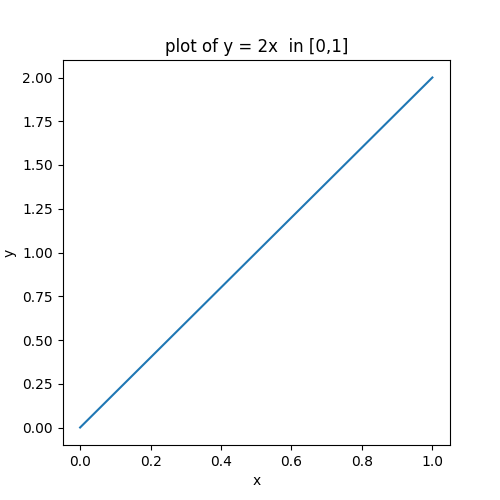
\includegraphics[width=0.7\textwidth]{images/chart_test}
\caption{نمونه‌ی استفاده از نمودار}
\label{chart:example}
\end{chart}

نمودار \ref{chart:example} نمونه‌ی استفاده از نمودار است.


\section{تعريف واژه‌ها (اختیاری)}
در این قسمت محقق باید واژه‌هایی که ممکن است برای خواننده آشنا نباشد تعریف کند


\section{خلاصه فصل‌ها}
در این قسمت خلاصه‌ای اشاره‌وار از فصل‌های آتی آورده می‌شود تا خواننده بتواند تصویری واضح از
دیگر قسمت‌های پایان‌نامه در ذهن خود ترسیم کند.

\clearpage

%  literature review chapter
\mainchapterstyle
\chapter{مروری بر مطالعات انجام شده}
\pagestyle{mainheader} 





\section{مقدمه}

هدف از این فصل که با عنوان‌های مروری بر ادبیات\LTRfootnote{Literature Review}، مروری بر منابع و یا مروری بر پیشینه تحقيق\LTRfootnote{Backgroung research} معرفی می‌شود، بررسی و طبقه‌بندی یافته‌های تحقیقات دیگر محققان در سطح دنیا و تعیین و شناسایی خلا‌های تحقیقاتی است. آنچه را که تحقیق شما به دانش موجود اضافه می‌کند، مشخص کنید. طرح پیشینه تحقیق\LTRfootnote{Backgroung Information} یک مرور محققانه است و تا آنجا باید پیش برود که پیش‌زمینه تاریخی مناسبی از تحقیق را بیان کند و جایگاه تحقیق فعلی را در میان آثار پیشین نشان دهد. برای این منظور منابع مرتبط با تحقیق را بررسی کنیدَ البته نه چندان گسترده که کل پیشینه تاریخی بحث را در برگیرد. برای نوشتن این بخش:

\begin{itemize} % example of itemize
  \item دانستنی‌های موجود و پیش‌زمینه تاریخی و وضعیت کنونی موضوع را چنان بیان کنید که خواننده بدون مراجعه به منابع پیشین، نتایج حاصل از مطالعات قبلی را درک و ارزیابی کند.
  \item نشان دهید که بر موضوع احاطه دارید. پرسش تحقیق را همراه بحث و جدل‌ها و مسائل مطرح شده بیان کنید و مهمترین تحقیق‌های انجام شده در این زمینه را معرفی نماید.
  \item ابتدا مطالب عمومی‌تر و سپس پژوهش‌های مشابه با کار خود را معرفی کرده و نشان دهید که تحقیق شما از چه جنبه‌ای با کار دیگران مطابقت یا تفاوت دارد.
  \item اگر کارهای قبلی را خلاصه کرده‌اید از پرداختن به جزئیات غیر ضروری بپرهیزید. در عوض بر یافته‌ها و مسائل روش شناختی مرتبط و نتایج اصلی تاکید کنید و اگر بررسی‌ها و منابع مروری عمومی درباره موضوع موجود است، خواننده را به آنها ارجاع دهید.
\end{itemize}


\section{تعاريف، اصول و مبانی نظری}
ارائه‌ی خلاصه‌ای از دانش کلاسیک موضوع است. این بخش الزامی نیست و بستگی به نظر استاد راهنما
دارد.
\begin{figure}[H] % example of using figures, you can change settings if required
\centering

\includegraphics[width=0.7\textwidth]{images/university-logo}
\caption{نمونه استفاده از شکل}
\label{fig:example}
\end{figure}

شکل \ref{fig:example} نمونه‌ای از استفاده از اشکال را نشان می‌دهد.

\section{مروری بر ادبیات موضوع}
در این قسمت باید به کارهای مشابه دیگران در گذشته اشاره کرد و وزن بیشتر این قسمت بهتر است به
مقالات ژورنالی سال‌های اخیر (2 تا 3 سال) تخصیص داده شود. نتایج کارهای دیگران همراه با ذکر دقیق
مراجع باید اشاره شده و جایگاه و تفاوت تحقیق شما نیز با کارهای دیگران مشخص شود. استفاده از مقالات
ژورنال‌های معتبر در دو یا سه سال اخیر می‌تواند به اعتبار کار شما بیافزاید.

نمونه‌ای از ارجاع به مقالات~\cite{fairoze2023publicly}. % example of citation to other researchs

\section{نتیجه‌گیری}
در نتیجه‌گیری آخر فصل، با توجه به بررسی انجام شده بر روی مراجع تحقیق، بخش‌های قابل گسترش و تحقیق در آن حیطه و چشم‌اندازهای تحقیق مورد بررسی قرار می‌گیرد. در برخی از تحقیقات، نتیجه نهایی فصل روش تحقیق، ارائه یک چارچوب کار تحقیقی\LTRfootnote{Research Framework} است.


\clearpage


%  literature review chapter
\mainchapterstyle
\chapter{روش تحقیق}
\pagestyle{mainheader} 


\section{مقدمه}
شرح کامل روش تحقیق است. این فصل بسته به نوع روش تحقیق و با نظر استاد راهنما می‌تواند مواد و روش‌ها\LTRfootnote{Materials and Methods}
نام گیرد. این فصل حدود 15 صفحه است.


\section{محتوا (نام گذاری بر اساس روش تحقیق و مسئله مورد مطالعه)}

\subsection{علت انتخاب روش}
دلیل یا دلایل انتخاب روش تحقیق را تشریح می‌کند.

\subsection{تشريح كامل روش تحقیق}
برای اینکه پایان‌نامه دارای ارزش علمی باشد، باید قابل تکرار باشد و داوران و خوانندگان از امکان
تکرارپذیر بودن کار شما مطمئن شوند. شما باید اساس تکرار آزمایش را به‌وسیله دیگران در این قسمت فراهم
کنید. تکرارپذیری آزمایشات و روش شما با میزان پتانسیل تکرار نتایج برابر یا نزدیک به آن است، در زیر به
تعدادی از روش‌های تحقیق اشاره شده است:

\begin{itemize}[leftmargin=*] % example of titled bullets

    \item \textbf{روش تحقیق مطالعه‌ی موردی} \\
    توصیف کامل برنامه‌ی آزمایشگاهی شامل مواد مصرفی و نحوه‌ی ساخت نمونه‌ها، شرح آزمایش‌ها شامل نحوه تنظیم و آماده‌سازی آزمایش‌ها و دستگاه‌های مورد استفاده و دقت و نحوه‌ی کالیبره کردن، شرح دستگاه ساخته شده (در صورت ساخت) و ارائه‌ی روش اعتبارسنجی.
    \item \textbf{روش تحقیق آماری} \\
    توصیف ابزارهای گردآوری اطلاعات کمی و کیفی، اندازه‌ی نمونه‌ها، روش نمونه‌برداری، تشریح مبانی روش آماری و ارائه‌ی روش اعتبارسنجی.
    \item \textbf{روش تحقیق نرم‌افزارنويسی} \\
    توصیف کامل برنامه‌نویسی، مبانی برنامه و ارائه‌ی روش اعتبارسنجی.

    \item \textbf{روش تحقیق مطالعه‌ی موردی} \\
    توصیف کامل محل و موضوع مطالعه، علت انتخاب مورد و پارامترهایی که تحت ارزیابی قرار داده می‌شوند، و ارائه‌ی روش اعتبارسنجی.
    \item \textbf{روش تحقیق تحلیلی يا مدل‌سازی} \\
    توصیف کامل مبانی یا اصول تحلیل یا مدل و ارائه‌ی روش اعتبارسنجی. در ارائه مدل ریاضی معمولا نیاز است اندیس ها، پارامترها، متغییرهای تصمیم و فرمول‌های مدل به صورت سیستماتیک ارائه شود. پیشنهاد می‌گردد برای نمایش اندیس ها، پارامتر‌ها و متغییرهای تصمیم از سه جدول به صورت زیر استفاده گردد.
    
    \begin{table}[h] % example of using tables
    \centering
    \caption{نمونه‌ی استفاده از جدول}
    \label{table:example}
    \begin{tabular}{cc}
    \hline
    ستون اول & ستون دوم \\
    \hline
    ۱ & ۲ \\
    \hline
    \end{tabular}
    \end{table}

    جدول~\ref{table:example} نمونه‌ای از استفاده از جدول را نشان می‌دهد در جدول \ref{longtable:example} هم میتوانید یک نمونه از جدول طولانی را ببینید


    \begin{longtable}{|c|c|c|} % example of using long table
    \caption{نمونه‌ی استفاده از جدول طولانی} \\
    \label{longtable:example}
    \hline
    ستون ۱ & ستون ۲ & ستون ۳ \\
    \hline
    \endfirsthead

    % ---------- continued title ----------
    \caption*{ادامه جدول \thetable} \\
    \hline
    ستون ۱ & ستون ۲ & ستون ۳ \\
    \hline
    \endhead

    % ---------- table body ----------
    داده & داده & داده \\
    \hline
    داده & داده & داده \\
    \hline
    داده & داده & داده \\
    \hline
    داده & داده & داده \\
    \hline
    داده & داده & داده \\
    \hline
    داده & داده & داده \\
    \hline
    داده & داده & داده \\
    \hline
    داده & داده & داده \\
    \hline
    داده & داده & داده \\
    \hline
    داده & داده & داده \\
    \hline
    داده & داده & داده \\
    \hline
    داده & داده & داده \\
    \hline
    داده & داده & داده \\
    \hline
    داده & داده & داده \\
    \hline
    داده & داده & داده \\
    \hline
    داده & داده & داده \\
    \hline
    داده & داده & داده \\
    \hline
    داده & داده & داده \\
    \hline
    داده & داده & داده \\
    \hline
    داده & داده & داده \\
    \hline
    داده & داده & داده \\
    \hline
    داده & داده & داده \\
    \hline
    داده & داده & داده \\
    \hline
    داده & داده & داده \\
    \hline
    داده & داده & داده \\
    \hline
    داده & داده & داده \\
    \hline
    داده & داده & داده \\
    \hline
    داده & داده & داده \\
    \hline
    داده & داده & داده \\
    \hline
    داده & داده & داده \\
    \hline
    داده & داده & داده \\
    \hline
    داده & داده & داده \\
    \hline
    داده & داده & داده \\
    \hline
    داده & داده & داده \\
    \hline
    داده & داده & داده \\
    \hline
    داده & داده & داده \\
    \hline
    داده & داده & داده \\
    \hline
    داده & داده & داده \\
    \hline
    داده & داده & داده \\
    \hline

    % ... many rows ...
    \end{longtable}

    \(\min(\delta_1, \delta)\)  نمونه‌ای از استفاده \lr{inline math} را نشان می‌دهد در حالی که در \ref{eq:sample} میتوانید نمونه‌ای از عبارات ریاضی را ببینید

    \begin{equation}
        \label{eq:sample}
        \bar{x} = \frac{\sum_{i=1}^{n} x_i}{n}
    \end{equation}


    همچنین در \ref{align:sample} خواهیم داشت:
    \begin{align}
    \label{align:sample}
    \mathbb{E}[Z] 
    &= \mathbb{E}[Z_{>\delta}] + \mathbb{E}[Z_{<\delta}] \\
    &\geq |I^{>\delta}| \cdot E_1 + |I^{<\delta}| \cdot \left(\frac{1}{2} - \frac{\mu\beta}{2}\right) \\
    &\geq p|y| \left[\frac{1}{2} + \left(\delta - \frac{1}{2}\right)\mu\beta\right] 
    + (1-p)|y| \left(\frac{1}{2} - \frac{\mu\beta}{2}\right) \\
    &= |y| \left[ \frac{1}{2} + p\delta\mu\beta - \frac{\mu\beta}{2} \right] \\
    &= \frac{|y|}{2} + \left(p\delta - \frac{1}{2}\right) \mu\beta |y|.
    \end{align}

    \item \textbf{روش تحقیق میدانی}\\
    چگونگی دستیابی به داده‌ها در میدان عمل و نحوه برداشت از پاسخ‌های دریافتی.

\end{itemize}



\begin{algorithm}[H] % example of using an algorithm
    \caption{\(\mathsf{Insertion Sort}(A)\)}
    \label{alg:inssort}
    \begin{algorithmic}[1]
        \REQUIRE آرایه \(A\)
        \ENSURE آرایه \(A\) در حالت مرتب شده
        \FOR{\(j = 2\) \TO \(A.length\)}
            \STATE \(key \gets A[j]\)
            \STATE \(i \gets j - 1\) \hfill // عنصر \(A[j]\) را در دنباله مرتب شده \(A[1,\ldots,j-1]\) درج کنید
            \WHILE{\(i > 0 \) \AND \(A[i] > key \)}
                \STATE \(A[i + 1] \gets A[i]\)
                \STATE \(i \gets i-1\)
            \ENDWHILE{}
            \STATE \(A[i + 1] \gets key\)
        \ENDFOR{}
        \RETURN \(A\)
    \end{algorithmic}
\end{algorithm}

الگوریتم~\ref{alg:inssort} نمونه‌ای از استفاده از یک الگوریتم را نشان می‌دهد.

\section{نتیجه‌گیری}
در این بخش نتیجه‌گیری فصل قرار می‌گیرد.
\clearpage

% expriments chapter
\mainchapterstyle
\chapter{تجزیه و تحلیل داده‌ها}
\pagestyle{mainheader}


\section{مقدمه}
ارائه‌ی داده‌ها، نتایج و تحلیل و تفسیر اولیه آنها در این فصل ارائه می‌شود. در ارائه‌ی نتایج با توجه به
راهنمای کلی نگارش فصل‌ها، تا حد امکان ترکیبی از نمودار و جدول استفاده شود. با توجه به حجم و ماهیت
تحقیق و با صلاحدید استاد راهنما، این فصل می‌تواند تحت عنوانی دیگر بیاید. در صورتی که حجم داده‌ها زیاد
باشد، بهتر است به صورت نمودار یا در قالب ضمیمه ارائه نشده و فقط نمونه‌ها در متن آورده شود. این فصل
باید به سوالات تحقیق عطف به یافته‌های محقق پاسخ داده شود. اگر تحقیق دارای آزمون فرض باشد، پذیرش
یا عدم پذیرش فرضیه‌ها در این فصل گزارش می‌شود. این فصل حدود 40 صفحه است.

\section{محتوا}
در این بخش به سوالات تحقیق براساس داده‌ها و یافته‌های محقق، پاسخ داده می‌شود.داده‌ها با فرمت
مناسبی ارائه می شوند. مدل‌ها اجرا شده و نتیجه آن مشخص می‌شود.

\section{اعتبارسنجی}
از طریق مقایسه نتایج با نتایج کارهای دیگران، استفاده از روش‌های تحلیل پایائی\LTRfootnote{Reliable} و اعتبار\LTRfootnote{Validity} ، نظرگیری از
خبرگان\LTRfootnote{Expert Judgment} انجام می شود.

\clearpage

% sample chapter

\mainchapterstyle
\chapter{بحث و نتیجه‌گیری}
\pagestyle{mainheader}

\section{مقدمه}
تاکنون شما در پایان‌نامه‌ای که مشغول نوشتن آن هستید، پاسخ چهار سؤال را دادهاید:
چرا تحقیق را انجام دادید؟ (مقدمه)
دیگران در این زمینه چه کارهایی کرده‌اند و تمایز کار شما با آنها چیست؟ (مرور ادبیات)
چگونه تحقیق را انجام دادید؟ (روش‌ها)
چه از تحقیق به دست آوردید؟ (یافته‌ها)
حال زمان آن فرا رسیده که با توجه به تمامی مطالب ذکر شده، در نهایت به سؤال آخر پاسخ دهید:
چه برداشتی از یافته‌های تحقیق کردید؟ (نتیجه‌گیری)
در واقع در این بخش، هدف پاسخ به این سؤال است که چه برداشتی از یافته‌ها کردید و این یافته‌ها چه
فایده‌ای دارند؟

نتیجه‌گیری مختصری بنویسید. ارائه‌ی داده‌ها، نتایج و یافته‌ها در فصل چهارم ارائه می‌شود. در این فصل
تفاوت، تضاد یا تطابق بین نتایج تحقیق با نتایج دیگر محققان باید ذکر شود. تفسایر و تحلیل نتایج نباید بر
اساس حدس و گمان باشد، بلکه باید برمبنای نتایج عملی استخراج شده از تحقیق و یا استناد به تحقیقات
دیگران باشد. با توجه به حجم و ماهیت تحقیق و با صلاحدید استاد راهنما، این فصل میتواند تحت عنوانی
دیگر بیاید یا به دو فصل جداگانه با عناوین مناسب، تفکیک شود. این فصل فقط باید به جمع‌بندی
دست‌آوردهای فصلهای چهارم و پنجم محدود و از ذکر موارد جدید در آن خودداری شود. در عنوان این فصل، به جای کلمه تفسیر می‌توان از واژگان بحث و تحلیل هم استفاده کرد. این فصل شاید مهم‌ترین فصل پایان‌نامه باشد.

در این فصل خلاصه‌ای از یافته‌های تحقیق جاری ارائه می‌شود. این فصل میتواند حاوی یک مقدمه،
شامل مروری اجمالی بر مراحل انجام تحقیق باشد (حدود یک صفحه). مطالب پاراگراف‌بندی شود و هر
پاراگراف به یک موضوع مستقل اختصاص یابد. فقط به ارائه‌ی یافته‌ها و دست‌آوردها بسنده شود و از تعمیم
بی‌مورد نتایج خودداری شود. تا حد امکان از ارائه‌ی جداول و نمودارها اجتناب شود. از ارائه‌ی عناوین کلی در
حوزه‌ی تحقیق و پیشنهاد تحقیقات آتی خودداری شود و کاملا در چارچوب و زمینه‌ی مربوط به تحقیق جاری
باشد. این فصل حدود 10 - 15 صفحه است.

\section{محتوا}
به ترتیب شامل موارد زیر است:

\subsection{جمع‌بندی}
خلاصه‌ای از تمام یافته‌ها و دست‌آوردهای تحقیق جاری است.

\subsection{نوآوری}
نوآوری تحقیق را بر اساس یافته‌های آن تشریح می‌کند. که دارای دو بخش اصلی است: نوآوری
تئوری، یعنی تمایز تئوریک کار با کارهای محققین قبلی و نوآوری عملی، یعنی توصیه های محقق به
صنعت برای بهبود بخشیدن به کارها بر اساس یافته های تحقیق.

\subsection{پیشنهادها}
عناوین و موضوعات پیشنهادی را برای تحقیقات آتی بیشتر در زمینه‌ی مورد بحث در آینده ارائه می‌کند.


\subsection{محدودیت‌ها}
محدودیت‌هایی که کنترل آن از عهده محقق خارج است مانند انتخاب نوع یافته‌ها و دیگر محدودیت‌هایی که کنترل آن در دست محقق است مانند موضوع و محل تحقیق و ... تشریح می‌شوند. تاثیر این
محدودیت‌ها بر یافته‌های تحقیق در این قسمت شرح داده می‌شوند.
\clearpage


\clearpage
\renewcommand{\bibname}{منابع و مراجع}
\bibliographystyle{apalike}

\makeatletter
\patchcmd{\thebibliography}
  {\chapter*{\bibname}}
  {%
    \chapter*{\bibname}%
    \addcontentsline{toc}{chapter}{\protect\BNazaninFont\bibname}%
    \latin\latinfont % ← switch bibliography body to Latin
  }
  {}{}
  \renewcommand{\@biblabel}[1]{\textbullet\ } % ← here is the bullet
\makeatother

\bibliography{references}


\clearpage
\chapter*{پیوست‌ها}                          % No chapter number
\addcontentsline{toc}{chapter}{\protect\BNazaninFont پیوست‌ها} % TOC entry

\appendix                                     % switches LaTeX to appendix mode

% Include appendix files here 
توجه مهم:
کلیه دانشجویان موظفند تمامی داده‌هایی که برای تهیه پایان‌نامه خود استفاده
نموده اند (شامل پرسشنامه ها، جداول آماری، کدنویسی ها، خروجی های نرم افزار
و ...  در انتهای پایان‌نامه به صورت پیوست ضمیمه کنند).
استثنا: دانشجویانی که پایان‌نامه آن‌ها به صورت کیفی (\lr{Qualitative}) می باشد، نیاز به ضمیمه کردن پیوست نخواهند داشت.
% extra appendices like appendix2.tex and etc.
\clearpage


% ---------- English Abstract ----------
\begin{latin}

% \thispagestyle{plain}
\thispagestyle{empty}

% ----- Abstract title (LEFT, not centered) -----
{\fontsize{13}{16}\selectfont\textbf{Abstract:}}

\vspace{24pt}

% ----- Abstract text -----
{\fontsize{12}{15}\selectfont
Lorem ipsum dolor sit amet, ea qui dico sententiae, ignota sententiae moderatius eu quo. Dicit moderatius id vis, omnes debitis epicuri ei mei, prima tamquam eu pro. Te vivendum sensibus efficiantur vis. Eripuit repudiare est et, exerci ancillae ut sed. Eum an malorum neglegentur, ad sea facilis vituperata argumentum. Qui sale fabulas vulputate no, et has vulputate accommodare, est no clita nominati oportere.
Dolor commodo signiferumque vix ad, decore oblique phaedrum sit ne. Propriae oporteat mel et, consul ceteros nec id. Te eum sale appetere, usu expetendis interesset id. Ius ut tation ancillae recteque, ei eam nulla postulant, affert postea scaevola ex eum.
}

\vspace{18pt}

% ----- Keywords -----
{\fontsize{12}{15}\selectfont\textbf{Keywords:}}
{\fontsize{12}{15}\selectfont
Mazim, altera, periculis, eu quo, iisque ullamcorper.
}

\vfill

% ----- Supervisor Signature -----
\begin{flushright}
{\fontsize{12}{14}\selectfont
Supervisor Signature
}
\end{flushright}

\end{latin}

\clearpage

% ---------- English Title Page ----------
\begin{latin}
\thispagestyle{empty}

\begin{center}

% ---------- University Logo ----------

\includegraphics[width=3cm]{images/university-logo}

\vspace{0.8cm}

% ---------- University Name ----------
{\fontsize{12}{14}\selectfont\textbf{KHATAM University}}\\
{\fontsize{12}{14}\selectfont\textbf{Non-governmental, Non-profitable}}

\vspace{1cm}

% ---------- Faculty ----------
{\fontsize{11}{13}\selectfont\textbf{Faculty of ......}}

\vspace{0.4cm}

% ---------- Department ----------
{\fontsize{10}{12}\selectfont\textbf{Department of ......}}

\vspace{1cm}

% ---------- Thesis Title ----------
{\fontsize{17}{20}\selectfont\textbf{Thesis title}}

\vspace{1cm}

% ---------- Degree Explanation ----------
{\fontsize{13}{16}\selectfont
A thesis submitted to the Graduate Studies Office\\
In partial fulfillment of the requirements for\\
The degree of M.Sc in ......
}

\vspace{0.7cm}

% ---------- First Supervisor ----------
{\fontsize{13}{16}\selectfont\textbf{First Supervisor:}}\\
{\fontsize{13}{16}\selectfont
Dr. ......
}

\vspace{0.7cm}

% ---------- Second Supervisor ----------
{\fontsize{13}{16}\selectfont\textbf{Second Supervisor:}}\\
{\fontsize{13}{16}\selectfont
Dr. ......
}

\vspace{0.7cm}

% ---------- Student ----------
{\fontsize{13}{16}\selectfont\textbf{By:}}\\
{\fontsize{13}{16}\selectfont
Student name
}

\vfill

% ---------- Date in format month year (e.g. April 2026)  ----------
{\fontsize{13}{16}\selectfont
...... 2026
}

\end{center}

\end{latin}

\clearpage

\end{document}